\documentclass[10pt]{reportMaster}

\usepackage[a4paper]{geometry}
\usepackage{acronym}
\usepackage{todonotes}
\usepackage{amsmath}
\usepackage{graphicx}
\usepackage{wrapfig}
\usepackage{bbold}
\usepackage[justification=centering]{caption}
\newcommand{\source}[1]{\caption*{Source: {#1}} }
\graphicspath{ {./images/} }
\DeclareMathOperator*{\argmax}{arg\,max}
\DeclareMathOperator*{\argmin}{arg\,min}

%%% The title of the thesis, and the author (astudent) of the thesis
\title{Learning Policies with Neural Ordinary Differential Equations}
\author{Lukas Schreiner}

%%% Uncomment the line with the Master program of the student
% \nameMastersProgramme{Data Science for Decision Making}  
\nameMastersProgramme{Artificial Intelligence}

%%% Here, write the department supervisor(s), as well as all department examiners; 
%%% Write also any external supervisor(s), if applicable
\committee{Prof. F. Thuijsman \\ Dr. P. Bonizzi \\ Elon Musk}
\date{September 22, 2022}


\begin{document}

\maketitle

\tableofcontents

\newpage

\section*{Table of abbreviations}

\begin{acronym}

\acro{RL}[RL]{Reinforcement learning}
\acro{NN}[NN]{neural network}
\acro{DRL}[DRL]{deep reinforcement learning}
\acro{NODE}[nODE]{neural ordinary differential equation}
\acro{ODE}[ODE]{ordinary differential equation}
\acro{MDP}[MDP]{markov decision process}
\acro{TD}[TD]{temporal difference}
\acro{SARSA}[SARSA]{State–Action–Reward–State–Action}
\acro{DQN}[DQN]{deep Q neural networks}
\acro{NFQ}[NFQ]{neural fitted Q iteration}

\end{acronym}

\newpage

\chapter{Introduction} \label{Introduction}

\ac{RL} is one of the major machine learning domains that experienced siginificant advances in recent years. An \ac{RL} agent learns through interaction with the environment and it's corresponding reward signals. Through try and error, the agent is able to explore new strategies and come up with novel solutions to solve the given problem. 

This fundamentally differentiates \ac{RL} from supervised and unsupervised learning techniques that rely on learning patterns from data. Some authors classify \ac{RL} as semi supervised. The key challenge is to learn a representation that gives guidance what the agent should do in each state it encounters. In early models this was done by a table that contained the action values for each state. This approach is obviously not feasible as the number of states and available actions increases since the table would grow exponentially and quickly exceed memory. A solution to this issue was to replace the table with a function that is represented by a \ac{NN}. The advantage is that a \ac{NN} can assign similar action values to states that have similar features, this technique is called \ac{DRL} \cite{mnih2013playing}. 

Recently, a new kind of \ac{NN} attracted a lot of attention. \ac{NODE}s use the \ac{NN} not for approximating function values directly but rather learn a differential equations for the inner state. The model output is then derived by solving an initial value problem with the learned \ac{ODE}. By discretising the \ac{NODE}, the hidden state of the model can have an arbitrary number of layers, which comes with numerous advantageous properties. This work aims to given a throughout assessment whether \ac{NODE}s are suited for being used in \ac{RL} problems, in particular, whether they exceed performance of conventional \ac{NN}s in a \ac{DRL} context. \\

The thesis is structured the following way. Chapter \ref{Introduction} gives an general and formal introduction to reinforcement Learning (section \ref{Reinforcement Learning}), deep reinforcement learning (section \ref{Deep Reinforcement Learning}) and neural ordinary differential equation (section \ref{Neural Ordinary Differential Equations}). Chapter \ref{Reinforcement Learning with neural ODEs} introduces the model and necessary adjustments needed for \ac{RL}. Chapter \ref{Reinforcement Learning with neural ODEs} describes the experimental set up before chapter \ref{Results} presents the empirical results from the experiments. Chapter \ref{Conclusion} closes with a conclusion and provides an outlook and perspective on further research. 

\newpage
\section{Reinforcement Learning} \label{Reinforcement Learning}

\paragraph{The Reinforcement Learning Problem} \ac{RL} is essentially a framework for learning how to interact with the environment from experience. The environment is thereby represented by a set of states $s \in S$ that the agents visits depending on the actions $a \in A$ played and optionally a random factor. In each state transition, the agent receives a reward signal $r(s, s', a)$ depending on the action played in current state and the resulting subsequent state. The agent now tries learn a policy $\pi(s, a)$ that maximises the total or average reward obtained. Since rewards occur in future states, the agent needs planning capabilities in order optimally solve the problem. In order to evaluate which action to choose the agent uses a state value function $V_{\pi}(s)$ that indicates what the discounted future rewards will be if the agent follows a given policy $\pi$. When learning, the agent faces the tradeoff whether to optimise the current strategy (on-policy) or try new random actions that might be suboptimal but lead to a higher reward in the future (off-policy). This is referred as the exploitation-exploration trade off in \ac{RL} \cite{march1991exploration}. There exists a rich body of literature of methods that aim to solve the \ac{RL} in various different ways. One of the main features that separates all is methods is whether the agent has a model of the environment available or not. If so, the agent can better asses the consequences of an action played yet coming up with a model of the environment is often not a trivial task for the researcher and so the recent literature mostly focuses on model-free approaches. See \cite{szepesvari2009reinforcement, sutton2018reinforcement} for an overview. 

\paragraph{Model-based reinforcement learning} If there exists a probabilistic model of the environment, the transition probability $t(s, a, s')$ and its corresponding reward function $r(s, a, s')$ between states are known. In this case the problem can be modelled using a \ac{MDP} \cite{bellman1957markovian}. If the state and action space are reasonable in size, one can either use value iteration or policy iteration in order derive an optimal policy $\pi^{*}(s)$. 
Value iteration is an algorithm that visits every state and chooses thereby the action that yields the highest Bellman update consisting of the the current reward plus the discounted future state value. After sufficient iterations, the optimal policy is derived by choosing the action in state the yields the highest state values

\begin{equation}
\label{eq:BellmanUpdateValueFunctionModelBased}
V_{\pi, new}(s_{t})= \max_{a}[r(s, a) + \gamma * \Sigma_{s}t(s, a, s')*V(s')], \text{ for } s \in S
\end{equation}

After convergence, the optimal policy is given by 

\begin{equation}
\label{eq:BellmanUpdateValueFunctionModelBasedconvergence}
\pi(s)^{*}= \argmax_{a}[r(s, a) + \gamma * \Sigma_{s}t(s, a, s')*V(s')], \text{ for } s \in S
\end{equation}

Policy iteration, on the other hand, computes the utility values $u(s, \pi)$ for all the states following the current policy $\pi(s)$ thereby evaluating the policy. 

\begin{equation}
\label{eq:utility value}
u(s, \pi) = r(s, \pi(s)) + \gamma * \Sigma_{s}t(s, \pi(s), s')u(s', \pi)), \text{ for } s \in S
\end{equation}

In a second step, the policy is improved until convergence $\pi_{new}(s) =\pi(s) = \pi(s)^{*}$

\begin{equation}
\label{eq:optimalpoliciy}
\pi_{new}(s) = \argmax_{a'}[r(s, \pi(s)) + \gamma \Sigma_{s}t(s, a', s') u(s', \pi)],  \text{ for } s \in S
\end{equation}


When doing policy iteration, the agent plays the action that the current policy intends for the given state. If the the action does not chooses the state transition that leads to the highest state value in the future state, the policy is updated. While being a mathematically sound theory, this approach is not suited for high dimensional state spaces since visiting all states of the environment for one update is can become computationally very expensive.

\paragraph{Model-free reinforcement learning} In many situations there does not exists a model of the underlying environment so the transition probabilities $t(s, a, s')$ are not known. In this case, the agent cannot compute an expected reward and needs to rely only on the reward signal of the actions played. In a naive monte carlo approach, the agent just plays through a whole episode of states and at the end of each episode the value function for visited states is updated with an average of the cumulated reward. While this approach is unbiased and will find an optimal policy at some point it is very sample inefficient.  

A more efficient way is therefore to use \ac{TD} learning \cite{sutton1988learning}, which updates the state values after a certain number of states are played. Thereby a \ac{TD} target estimate is computed by summing the current reward $r_{t}$ with the $\gamma$ discounted state value estimates ranging some states into the future. How those future states and actions are determined depends on the specific learning algorithm used. The difference between the \ac{TD} target estimate and the old function estimate is called \ac{TD} error and is used to update the function after being multiplied with the learning rate $\alpha$. In TD(0) this means that only the next state is considered which gives an update rule for the value function

\begin{equation}
\label{eq:bellman update value function}
V_{new}(s_{t})= V_{new}(s_{t}) + \alpha * \overbrace{(\underbrace{r_{t} + \gamma V_{old}}_{\text{TD estimate}} - V_{old})}^{\text{TD error}}
\end{equation}

While the value function $V(s)$ gives the state value assuming the agent plays the best action, the Q-function $Q(s, a)$ gives back the state value for any action that the agent could play. This richer representation of state values is therefore well suited for explorative off policy algorithms. The optimal policy is then derived by choosing the action that yields the highest Q-value in a given state $\pi(s, a)=\argmax_{a}Q(s, a)$. There are two main domains for learning the Q-function, on-policy algorithms like \ac{SARSA} \cite{rummery1994line} that learns by strictly following the policy $\pi(s_{t})=a_{t}$.

\begin{equation}
\label{eq:bellman update SARSA}
Q_{new}(s_{t}, a_{t})= Q_{old}(s_{t}, a_{t}) + \alpha * (r_{t}(s, a) + \gamma Q_{old}(s_{t+1}, a_{t+1}) - Q_{old}(s_{t}, a_{t}))
\end{equation}


Q-learning \cite{watkins1992q} is an off-policy learning algorithm because it mixes playing random actions (exploration), and following the reward maximising policy (exploitation). In both cases the Q-values are updated using a bellman equation 

\begin{equation}
\label{eq:q-learning}
Q_{new}(s_{t}, a_{t})= Q_{old}(s_{t}, a_{t}) + \alpha * (r_{t}(s, a) + \gamma \max_{a}Q_{new}(s_{t+1}, a) - Q_{old}(s_{t}, a_{t}))
\end{equation}

This allows the agent not only learn not only from imitation but also from experience replay \cite{lin1992self}. Thereby the agent samples past state transitions in order to improve the Q-values. Q-learning tends to convergence faster than \ac{SARSA} yet it incorporates higher variance. In practice, starting with a lot of off-policy exploration and then transitioning into on-policy learning works well for many problems. Usually an $\epsilon$-greedy algorithm is used that represents a decreasing probability threshold that determines whether a random action is played or the agent should follow the policy. See \cite{sutton2018reinforcement} for an extensive overview. 

\newpage
\section{Deep Reinforcement Learning} \label{Deep Reinforcement Learning}

As already mentioned, storing value functions and policies in tables is only feasible when the action and state space is of limited size. For that reason the logical next step was to learn a function that represents the value function \cite{sutton1999policy}. This way, not only \ac{RL} problems with large state and action spaces could be solved, but it also could leverage the fact that some states are very similar in attributes and therefore have similar optimal actions. 

Even though the idea to use neural networks as function approximation is rather old \cite{bertsekas1996neuro}, the breakthrough occurred with \ac{DQN} \cite{mnih2013playing} and AlphaGo \cite{silver2016mastering}. Deep reinforcement learning is very powerful but it comes with new challenges regarding convergence \cite{tsitsiklis1996analysis}. The combination of non linear function approximation, experience replay and off-policy learning might cause the divergence in function approximation. In order to introduce stability into the function approximation setting, multiple approaches exist. All of them try to reduce the chance that suboptimal actions get overestimated and consequently selected too often which causes the model to diverge. 

The \ac{NFQ} algorithm \cite{riedmiller2005neural} does not update network weights after each environment step but rather considers a the entire set of transition experiences. While this approach yields more stable results convergence is slow. 
\ac{DQN}s find a suitable balance between stability and convergence by using a target and policy \ac{DQN} network. While the weights of the policy net are updated after each enviroment step, the target network is used to select the actions. Every $c$ steps the target net is updated with a copy of the weights of the policy net. Double \ac{DQN}s \cite{hasselt2010double} use two networks and the action is selected with a $50\%$ chance by each of them. An updated version of this algorithm uses one network for action selection and the other one action evaluation. The weights of the former network are updated similar to an exponentially weighted moving average \cite{van2016deep}. 

Another way of reducing the risk of overestimating is using prioritised experience replay \cite{schaul2015prioritized}, which samples state transitions according to their experienced \ac{TD} error. That way, state transitions that yield a higher learning effect are sampled more often. Stochastic sampling ensures that probabilities are interpolated between a pure greedy approach and conventional uniform sampling. That allocates a nonzero probability to each transition and prevents overfitting. 

Double Q Networks have since then contributed to advances in many fields, e.g. for automomous \cite{zhang2018human} as well as well as electric \cite{chen2022energy} vehicles but also nuclear \cite{liu2019double}, quantum \cite{he2021variational} and IoT \cite{li2020onboard} applications. 

\newpage
\section{Neural Ordinary Differential Equations} \label{Neural Ordinary Differential Equations}


\begin{wrapfigure}{L}{0.4\textwidth}
\centering
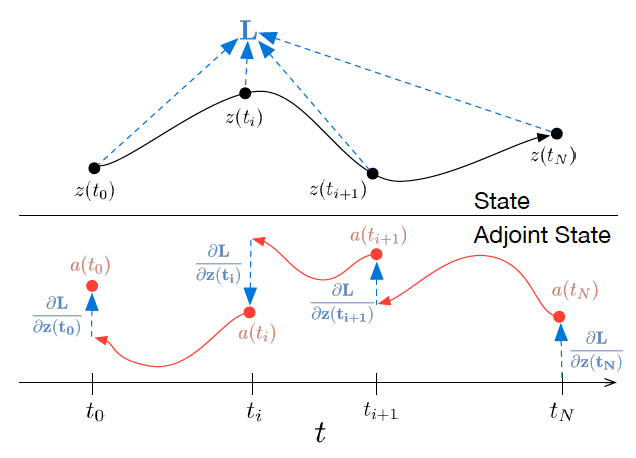
\includegraphics[width=6cm]{ContinuousBackProp}
\caption{Continuous Backpropagation \cite[Figure 2]{chen2018neural}}
\label{fig:ContinuousBackProp}
\end{wrapfigure}

Neural ordinary differential equations \cite{chen2018neural} are a novel method for deep learning that follow a different approach. While conventional feed forward neural networks learn a function that maps the input vector $x$ and model parameter $\theta$ to the model output $\tilde{y}$ ($f(x, \theta)=\tilde{y}$), \ac{NODE}s use the neural network to learn a differential function that describes the hidden state $z(t)$.

\begin{equation}
\label{eq:NeuralNetworkAsHiddenStateDynamics}
f(z(t), t, \theta) = \frac{dz(t)}{dt}
\end{equation}

The model output is then determined by solving an initial value problem using the model input as starting point at $t_{0}$ solving for the value at $t_{N}$. That way, the hidden state is continuous in the limit and discretised by the evaluation points at $t_{0}, t_{i}, t_{i+1}, \ldots, t_{N} $  by the ODE solver. The loss is then computed as the solution of the solver which defines the loss function $L$ as follows 

\begin{equation}
\label{eq:loss function}
L(z(t_{1})) = L(z(t_{0}) + \int_{t_{0}}^{t_{1}}f(z(t), t, \theta)) = L(ODESolve(z(t_{0}), f, t_{0}, t_{1}, \theta))
\end{equation}
 
Thereby $z(t_{1})$ is the hidden state at $t_{1}$ and represents the model output. In order to learn the parameters $\theta$ of the neural network, the authors suggest to use the adjoint method \cite{pontryagin1987mathematical} which defines an adjoint ODE that is solved backwards in time, see figure \ref{fig:ContinuousBackProp}.

\paragraph{Continuous Backpropagation}

In order to compute the gradients with respect to the weights $\frac{dL}{d\theta}$, an adjoint state $a(t)$ is defined as the the gradient of the hidden state with respect to to the loss, see \ref{eq:adjointstate}.  That avoids backpropagating though the ODE solver. The dynamics of $a(t)$ are derived by making use of the definition of the neural network's hidden state  through time $\frac{dz(t)}{dt}$ and the chain rule. The derivations follow \cite[Appendix B.1]{chen2018neural}. 

\begin{align}
a(t) = & \frac{d L}{d z(t)} = \frac{d L}{d z(t + \epsilon)} \frac{d z(t + \epsilon)}{dz(t)}  \label{eq:adjointstate} \\
a(t +\epsilon) = & \frac{d L}{d z(t + \epsilon)}   \label{eq:adjointstateepsilon}
\end{align}

The finite difference of the hidden state is then given by

 \begin{equation}
\label{eq:hiddenstatedynamicsespsilon}
z(t + \epsilon) =  \int_{t}^{t + \epsilon} f(z(t), t, \theta)dt + z(t) = T_{\epsilon}(z(t), t)
\end{equation}

which can be shown by transforming and integrating \ref{eq:NeuralNetworkAsHiddenStateDynamics}. Plugging \ref{eq:hiddenstatedynamicsespsilon} and \ref{eq:adjointstateepsilon} into \ref{eq:adjointstate} gives

\begin{equation}
\label{eq:adjointstatedefinition}
a(t) = a(t+\epsilon) \frac{\partial T_{\epsilon}(z(t), t)}{\partial z(t)}
\end{equation}

The dynamics of $a(t)$ is then derived using the definition of a derivative coming from finite differences in the limit.

\begin{equation} \begin{split}
\label{eq:adjstate} 
\frac{da(t)}{dt}
& =  \lim_{x \to 0^{+}}  \frac{a(t+\epsilon) - a(t)}{\epsilon}\\
& =  \lim_{x \to 0^{+}}  \frac{a(t+\epsilon) - a(t+\epsilon) \frac{\partial T_{\epsilon}(z(t), t)}{\partial z(t)}}{\epsilon}\\
& =  \lim_{x \to 0^{+}} \frac{a(t+\epsilon) - a(t+\epsilon) \frac{1}{\partial z(t)} (z(t) + \epsilon f(z(t), t, \theta) + \mathcal{O}(\epsilon^{2}))}{\epsilon} \\
& =  \lim_{x \to 0^{+}} \frac{a(t+\epsilon) - a(t+\epsilon) (\mathit{I} + \epsilon \frac{f(z(t), t, \theta)}{dz(t)} + \mathcal{O}(\epsilon^{2}))}{\epsilon} \\
& =  \lim_{x \to 0^{+}} \frac{-a(t+\epsilon) \epsilon \frac{f(z(t), t, \theta)}{dz(t)} + \mathcal{O}(\epsilon^{2})}{\epsilon} \\
& =  \lim_{x \to 0^{+}} -a(t+\epsilon) \frac{f(z(t), t, \theta)}{dz(t)} + \mathcal{O}(\epsilon^{1})\\
\end{split}
\end{equation}

which in the limit gives

\begin{equation}
\label{eq:adjointstatedynamicsdefinition}
\frac{da(t)}{dt} = -a(t)^{T} \frac{f(z(t), t, \theta)}{dz(t)}\\
\end{equation}

with \ref{eq:adjointstatedynamicsdefinition} being one of the key results in the paper. The gradient at the final value $t_{N}$ and model output is defined by 

\begin{equation}
\label{eq:adjointstatefinalvalue}
a(t_{N}) =  \frac{dL}{dz(t_{N})}\\
\end{equation}

from which we can derive the the gradient with respect to to the hidden state at any point in time including the initial or input value. 

\begin{equation}
\label{eq:adjointstateanyvalue}
a(t_{0}) =  \frac{dL}{dz(t_{0})} + \int_{t_{N}}^{t_{0}} \frac{da(t)}{dt}dt = a(t_{N}) -  \int_{t_{N}}^{t_{0}} a(t)^{T} \frac{\partial f(z(t), t, \theta)}{\partial z(t)} \\
\end{equation}

In \ref{eq:adjointstateanyvalue}, it is assumed that the loss $L$ depends only on the last time point $t_{N}$. If the loss function also should depend on intermediate steps $t_{1}, t_{2}, t_{3}, ...$, the adjoint step is repeated backward for the intervals $[t_{N-1}, t_{N}], [t_{N-2}, t_{N-1}], ...$ with the gradients added together at the end. 

\paragraph{Gradients for the model parameters} 

In order to derive the gradients with respect to the parameters of the model, the authors generalise \ref{eq:adjointstatedynamicsdefinition} by defining the adjoint state as a vector consisting of the hidden state $z$, the model parameters $\theta$ as well as the time dimension $t$, see \cite[Appendix B.2]{chen2018neural}. Since the model parameters are a constant and $t$ is constant with respect to itself, the time dynamics are given by 

\begin{equation}
\label{eq:timedynamicstheta}
 \frac{\partial \theta(t)}{dt} = 0 \\
\end{equation}

\begin{equation}
\label{eq:timedynamicst}
 \frac{\partial t(t)}{dt} = 1 \\
\end{equation}

Using  \ref{eq:NeuralNetworkAsHiddenStateDynamics},  \ref{eq:timedynamicstheta} and \ref{eq:timedynamicst} and the combined time dynamics is then given by

\begin{equation}
\label{eq:timedynamicscombinedaugmentedstate}
\frac{d}{dt}
\begin{bmatrix}
z \\
\theta \\
t \\
\end{bmatrix} = f_{aug}([z, \theta, t]) : =
\begin{bmatrix}
f([z, \theta, t]) \\
0 \\
1 \\
\end{bmatrix}
\end{equation}

The jacobian of $f_{aug}$ is 

\begin{equation}
\label{eq:fjacobian}
\frac{\partial f_{aug}}{\partial [z, \theta, t]} = 
\begin{bmatrix}
\frac{\partial f_{aug}}{\partial z} & \frac{\partial f_{aug}}{\partial \theta}  & \frac{\partial f_{aug}}{\partial t} \\
\textbf{0} & \textbf{0} & \textbf{0} \\
\textbf{0} & \textbf{0} & \textbf{0} \\
\end{bmatrix}
\end{equation}

with \textbf{0} being matrices of zeros that have corresponding shapes depending on $\theta$ and $t$. The combined augmented state is defined as follows with the first element in the vector being similar to \ref{eq:adjointstate}

\begin{equation}
\label{eq:combinedaugmentedstate}
a_{aug} := 
\begin{bmatrix}
a \\
a_{\theta} \\
a_{t} \\
\end{bmatrix} = 
\begin{bmatrix}
\frac{dL}{dz(t)} \\
\frac{dL}{d\theta(t)}  \\
\frac{dL}{dt(t)}  \\
\end{bmatrix}
\end{equation}

With its dynamics given by \ref{eq:adjointstatedynamicsdefinition}

\begin{equation}
\label{eq:combinedaugmentedstatedynamics}
 \frac{da_{aug}(t)}{dt} = -a_{aug}(t)^{T} \frac{\partial f_{aug}}{\partial [z, \theta, t]} (t) \\
\end{equation}

Finally, \ref{eq:fjacobian} and \ref{eq:combinedaugmentedstate}  plugged into \ref{eq:combinedaugmentedstatedynamics} yields

\begin{equation}
\label{eq:combinedaugmentedstatedynamicsfinal}
 \frac{da_{aug}(t)}{dt} 
 = 
 -  \begin{bmatrix}
 a & a_{\theta} & a_{t}
  \end{bmatrix}
  \begin{bmatrix}
 \frac{\partial f_{aug}}{\partial z} & \frac{\partial f_{aug}}{\partial \theta}  & \frac{\partial f_{aug}}{\partial t} \\
\textbf{0} & \textbf{0} & \textbf{0} \\
\textbf{0} & \textbf{0} & \textbf{0} \\
  \end{bmatrix} (t)
 =
-  \begin{bmatrix}
 a\frac{\partial f_{aug}}{\partial z} & a \frac{\partial f_{aug}}{\partial \theta} & a \frac{\partial f_{aug}}{\partial t}  \\
 \end{bmatrix} (t)\\
\end{equation}

with the first element in the vector being equal to \ref{eq:adjointstatedynamicsdefinition}. Similar to \ref{eq:adjointstateanyvalue}, the gradients with respect to the model parameters $\theta$ can be obtained by integrating the second element of the vector in \ref{eq:combinedaugmentedstatedynamicsfinal} over the full interval while setting $a_{\theta}(t_{N}) =  \textbf{0}$

\begin{equation}
\label{eq:gradientmodelparameters}
 \frac{\partial L}{d\theta} = a_{\theta}(t_{0}) = - \int_{t_{N}}^{t_{0}} a(t)^{T} \frac{\partial f(z(t), t, \theta)}{\partial \theta} dt\\
\end{equation}


\paragraph{Characteristics and applications of NODEs}

\todo{Claims from the authors}

Normalising Flows \cite{rezende2015variational}

\chapter{Reinforcement Learning with neural ODEs} \label{Reinforcement Learning with neural ODEs}

This work is mainly concerned with applying neural \ac{NODE}s to reinforcement learning problems and comparing their performance with regard to convergence, stability and overall reward achievements to a state of the art \ac{DQN} model of similar size. \\

Like conventional \ac{ODE}s, neural \ac{ODE} can only map input $x$ of similar dimensionality $\phi: \mathbb{R}^{d} \rightarrow \mathbb{R}^{d} $. That poses a major issue for their use \ac{DRL} because the agent is required to learn a mapping from a $d$ dimensional observation space to a $n$ dimensional action space. Common approaches either augment the input vector with a number of zeros such that dimensions match \cite{dupont2019augmented} or add a linear layer at the end of the \ac{NODE} \cite{lin2018resnet}. It has been shown that the latter architecture for ResNet \cite{jian2016deep} is a universal approximator \cite{lin2018resnet} and since ResNet are the contionous analogs of \ac{NODE}s \cite{sander2022residual}, this architecture is chosen in order to deal with dimensionality. See figure \ref{fig:nODEArchitecture} for an example with a one dimensional action space. 

\begin{wrapfigure}{L}{0.35\textwidth}
\centering
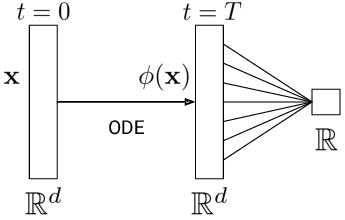
\includegraphics[width=5cm]{nODEArchitecture}
\caption{nODE architecture  \cite[Figure 2]{dupont2019augmented}}
\label{fig:nODEArchitecture}
\end{wrapfigure}

\paragraph{Hypothesis} 
One hypothesis to be examined is that the continuous nature of neural \ac{NODE}s might give them advantages in environments with action spaces that are continuous in nature. 

\paragraph{Model Set up} 

\todo{Dual model, prioritised experience replay, epsilon greedy}

\begin{wraptable}{r}{5.5cm}


\label{tab:model-hyperparameter}
\begin{tabular}{lll}
Description              & Value   &  \\ \cline{1-2}
Learning rate            & $l=0.001$ &  \\
Discount factor          & $\gamma =0.95$  &  \\
Target net weight update & $ \tau=0.05$  &  \\
Batch size               & $b=128$     &  \\
Epsilon greedy start    & $\epsilon_{0}=1.0$   &  \\
Epsilon greedy end       & $\epsilon_{N}=0.0$   & \\
No. Episodes       & $N = 2000$   & \\
\end{tabular}
\centering
\caption{Model Hyperparameter}
\end{wraptable}

\paragraph{Problem Setting} An experimental set up is created that simulates a \ac{DRL} problem, which is often referred to in the literature as the balancing pole \cite{barto1983neuronlike} problem. The agent controls a cart that can go to the left or to the right in a limited space. The cart has a horizontal pole attached on a joint and the agent receives a reward of 1 for each time step where the pole is balances in a somewhat upright position on the cart. If the pole tilts or the maximum number of 500 time steps is reached, the episode ends. The implementation used in this work comes from OpenAI's Gym library \cite{gymref}. A detailed description of the problem can be found in appendix \ref{Balancing Pole Appendix}.

\paragraph{Set up} In order to compare model performance, a conventional deep learning model is compared to neural ODE model with similar parameters are trained. In both set ups, are dual model set up is used with a policy and and target net \cite{hasselt2010double} with prioritised experience replay \cite{schaul2015prioritized}. First the models are trained evaluated under different conditions with different metrics. On the one hand, the speed of convergence is evaluated by measuring the number of episodes it takes the model to solve the environment for the first time while training. On the other hand, model robustness is tested by letting the model play the environment with different levels of distortions. 

\chapter{Results} \label{Results}

\chapter{Conclusion} \label{Conclusion}

\section{Outlook} \label{Outlook}

\bibliographystyle{plain}
\bibliography{refs}

\appendix

\chapter{Experimental Set Up}

\section{Balancing Pole} \label{Balancing Pole Appendix}

The action space of the balancing pole problem is discrete and consists of 2 possible actions. 

\begin{table}[h]
\centering
\label{tab:actions-bp}
\begin{tabular}{ll}
\multicolumn{1}{c}{\textbf{Num}} & \multicolumn{1}{c}{\textbf{Action}} \\ \hline
0                                & Push cart to the left               \\
1                                & Push cart to the right             
\end{tabular}
\end{table}

The observation space is four dimensional and covers position and velocity of the cart as well as the pole. 

\begin{table}[h]
\centering
\label{tab:observations-bp}
\begin{tabular}{lll}
\multicolumn{1}{c}{\textbf{Observation}} & \multicolumn{1}{c}{\textbf{Min}} & \multicolumn{1}{c}{\textbf{Max}} \\ \hline
Cart Position                            & $-4.8     $                        & $4.8        $                      \\
Cart Velocity                            & $-\inf$                             & $\inf$                              \\
Pole Angle                               & $\sim$ -0.418 rad (-24$^{\circ}) $         & $\sim$0.418 rad (24$^{\circ}) $           \\
Pole Angular Velocity                    & $-\inf$                             & $\inf$                             
\end{tabular}
\end{table}

The environment yields a reward of one for each time step, where the cart is still balancing the pole and it's position is still within the observation space. After a maximum of 500 time steps, the game stops resulting in a maximum reward of 500 per episode. 
\end{document}

